\documentclass[a4paper, 12pt]{article}

%\usepackage{config}

% page margin 
\usepackage[
top=2cm,
right=2.5cm,
bottom=2cm,
left=2.5cm
]{geometry}

% language and characters
\usepackage[utf8]{inputenc}
\usepackage[T1]{fontenc}
\usepackage[brazilian]{babel}
\usepackage{indentfirst	}
\usepackage{
	amsmath,
	amsfonts,
	amssymb
}

% colors
\usepackage{xcolor}
\usepackage{float}

% watermark config
\usepackage{xwatermark}
%\newwatermark[allpages, scale=4, angle=60, color=red!30]{text}

% equations numbering
\numberwithin{equation}{section}

% graphics insertion
\usepackage{graphicx}
\usepackage{subfig}

% references in the document (for equations, sections, images, websites)
\usepackage{hyperref}
\usepackage[]{cleveref}

\usepackage{siunitx}

% manual draw
\usepackage{tikz}

\begin{document}
	\begin{titlepage}
		\begin{center}
			\textbf{\href{https://www.unicamp.br/unicamp/}{Universidade Estadual de Campinas}}\\\vspace{1cm}
			\href{https://www.feagri.unicamp.br/portal/}{Faculdade de Engenharia Agrícola}\\\vspace{5cm}
			%\textbf{}\\\vspace{1cm}
			\large{Trabalho Final de FA622}\\\vspace{4cm}
		\end{center}
		
		\hspace{8cm}\parbox{7cm}{Relatório apresentado como parte da avaliação da disciplina FA622 - Sistema Solo-Planta-Atmosfera, sob responsabilidade do Prof. Dr. José Teixeira}\\\vspace{4cm}
		
		RENAN DA SILVA GUEDES - 223979\\\vspace{4cm}
		\begin{center}
			CAMPINAS - SP\\\vspace{.2cm}
			AGOSTO
		\end{center}
		
	\end{titlepage}

	\newpage
	
	\tableofcontents
	\listoffigures
	
	\newpage
	
	\section{Introdução}

	A seguir temos um estudo referente às características de transpiração apresentadas pelas folhas de diferentes espécies vegetais. Com base nos gráficos, é possível analisar a transpiração foliar (E), o déficit de pressão de vapor (DPV) e a radiação fotossinteticamente ativa (PAR). Com bases nesses parâmetros foi possível obter os dados em diferentes instantes de tempo e potenciais hídricos das plantas ($\Psi_{\textrm{pd}}$) como é visto na legenda.

	\subsection{Cana de açúcar}	
	A primeira parte do estudo diz respeito à cana de açúcar variedade RB67515. Para a mesma a coleta de dados foi feita em duas datas, sendo a primeira em 17/08/2015 e a segunda em 19/10/2015 (Figuras 1 e 2). Com base nisso, nota-se que as duas coletas objetivaram a aquisição de dados em duas condições ambientais diferentes, permitindo comparar a variação dos parâmetros referidos com base em tal mudança.
	
	Quando analisamos a transpiração das plantas de cana nota-se que na primeira data -- 17/08/15 -- a taxa de transpiração foi menor em média quando comparado ao dia 19/10/15. Isso demonstra que a planta com maior potencial hídrico ($\Psi_{\textrm{pd}}=\SI{-0.14}{\mega\pascal}$) obteve a maior taxa de transpiração ($\textrm{E}$ por volta de $\SI{8.5}{\milli\mole\cdot\meter^{-2}\cdot\second^{-1}}$). Entretanto, ao analisar o intervalo entre as 10h00 e 14h00 vê-se que a região onde ocorreu estabilização da taxa estava ao potencial de \SI{-.16}{\mega\pascal}, no dia 19/10/15, correspondendo a $\SI{2.85}{\milli\mole\cdot\meter^{-2}\cdot\second^{-1}}$ de E. Quando é feita a mesma análise para o dia 17 temos que para $\Psi_{\textrm{pd}}=\SI{-0.18}{\mega\pascal}$ o valor de E foi de $\SI{2.56}{\milli\mole\cdot\meter^{-2}\cdot\second^{-1}}$, demonstrando que a redução do $\Psi_{\textrm{pd}}$ é proporcional ao valor de E. 
	
	No que diz respeito à radiação fotossinteticamente ativa (PAR), vê-se que no dia 19 as médias dos valores de PAR para diferentes indivíduos são bem próximas, colaborando para o padrão de curvas sobrepostas observado. Todavia, para o dia 17 ao potencial de \SI{-18}{\mega\pascal} houve menor tendência de sobreposição. Nota-se que o maior valor de PAR ocorre para menores valores de potencial -- dia 17, correspondendo a $\SI{2010.50}{\micro\mole\cdot\meter^{-2}\cdot\second^{-1}}$ às 13h00.
	
	\subsection{Pata de vaca}
	Para a espécie pata de vaca, chegou-se que sob diferentes potenciais hídricos o maior valor de transpiração ocorreu entre as 12h00 e 14h00 em 28/11/16 correspondendo a $\SI{15.4}{\milli\mole\cdot\meter^{-2}\cdot\second^{-1}}$. Em contrapartida, ao meio dia desta data a menor respiração ocorreu para o menor potencial $\Psi_{\textrm{pd}}=\SI{-0.13}{\mega\pascal}$. Isso demonstra que nos momentos onde há maior incidência de luz solar o maior potencial hídrico colabora para a maior taxa de E.
	
	De maneira análoga, ao tomar como base PAR em função do tempo para a mesma espécie, tem-se que do período das 10h00 às 14h00 o menor valor de PAR foi identificado na última aferição, onde ao potencial de \SI{-.013}{\mega\pascal} obteve-se $\textrm{PAR}=\SI{717.3}{\micro\mole\cdot\meter^{-2}\cdot\second^{-1}}$. De todos os potenciais observados (\SI{-.09}{\mega\pascal}, \SI{-.10}{\mega\pascal}, \SI{-.11}{\mega\pascal} e \SI{-.13}{\mega\pascal}) a maior radiação fotossinteticamente ativa se deu ao meio dia, com $\Psi_{\textrm{pd}}=\SI{-0.09}{\mega\pascal}$ e $\SI{1890}{\micro\mole\cdot\meter^{-2}\cdot\second^{-1}}$, aproximando-se ligeiramente dos $\SI{1850.3}{\micro\mole\cdot\meter^{-2}\cdot\second^{-1}}$ observados para o potencial de \SI{-.10}{\mega\pascal}.
	
	Com relação ao DPV, para todos os potenciais hídricos nota-se sobreposição do DPV em função do tempo, de modo que os valores em \SI{}{\kilo\pascal} chegam a coincidir das 8h00 às 17h00. Para a última aferição -- 18h00 -- os valores destoaram por volta de \SI{0.5}{\kilo\pascal} entre o menor e o maior DPV registrado.
	
	\subsection{Myrtaceae}
	
	Para essa espécie, obteve-se que a maior taxa de transpiração ocorreu para o maior potencial hídrico ($\Psi_{\textrm{pd}}=\SI{-0.09}{\mega\pascal}$), dessa forma, foi observado um valor de $\textrm{E}=\SI{1747.8}{\milli\mole\cdot\meter^{-2}\cdot\second^{-1}}$. Em oposição, quando é considerado o menor potencial ($\Psi_{\textrm{pd}}=\SI{-0.12}{\mega\pascal}$) nota-se a ocorrência de duas quedas abruptas na E no intervalo entre as 8h00 e 14h00. É possível notar que para as mesmas foram responsáveis período, sendo que ao meio dia foi atingido um valor de $\textrm{E}=\SI{4}{\milli\mole\cdot\meter^{-2}\cdot\second^{-1}}$ que se estabilizou até às 15h00 em 30/11/2016.
	
	De maneira análoga, para a PAR o maior obtido se deu em $\Psi_{\textrm{pd}}=\SI{-0.11}{\mega\pascal}$ -- próximo ao menor potencial -- de modo que a intensidade aferida foi de $\SI{1858}{\micro\mole\cdot\meter^{-2}\cdot\second^{-1}}$ às 8h00. Entretanto, para o mesmo $\Psi_{\textrm{pd}}$ às 12h00 foi observada uma 
	$\textrm{PAR}=\SI{226.8}{\micro\mole\cdot\meter^{-2}\cdot\second^{-1}}$ -- menor de todo o período.	
	
	No caso do déficit de pressão de vapor, ao comparar com a espécie anteriormente analisada -- pata de vaca -- tem-se um comportamento muito similar entre ambas, diferenciando-se somente para a última medida realizada. A escala dos DPVs em função do tempo também se manteve, de modo que a sobreposição se repetiu com valores próximos em \SI{}{\kilo\pascal} em ambas as plantas.
	
	\subsection{Grumixama}
	
	A grumixama quando analisada nos três quesitos -- E, PAR e DPV -- apresenta um padrão que se distancia da uniformidade apresentada para as outras espécies, principalmente nas duas primeiras grandezas. Com base na respiração coletada dos indivíduos percebe-se uma ascensão da taxa respiratória às 10h00 em 03/12/2013. Para o menor potencial hídrico -- \SI{-.92}{\mega\pascal} -- é notado menor valor de E, sendo a transpiração igual a $\SI{.39}{\milli\mole\cdot\meter^{-2}\cdot\second^{-1}}$, bem distante dos $\SI{5.27}{\milli\mole\cdot\meter^{-2}\cdot\second^{-1}}$ obtidos para o mesmo horário com $\Psi_{\textrm{pd}}=\SI{-0.36}{\mega\pascal}$. Dessa maneira, com base no que foi visto, seria normal apontar o potencial hídrico atuando como fator limitante da respiração, ao afetar de modo proporcional E. Todavia, ao comparar a planta com o segundo menor potencial estudado (\SI{-.78}{\mega\pascal}), para o mesmo horário -- 10h00 -- foi aferida a terceira maior taxa de transpiração do período entre as 5h00 e 19h00 ($\textrm{E}=\SI{4.11}{\milli\mole\cdot\meter^{-2}\cdot\second^{-1}}$).
	
	Com base no gráfico (b) da Grumixama, nota-se que o comportamento das aferições demonstrou alta intermitência, por conta disso, independentemente do potencial hídrico (\SI{-.92}{\mega\pascal}, \SI{-.78}{\mega\pascal}, \SI{-.35}{\mega\pascal}, \SI{-.39}{\mega\pascal}, \SI{-.36}{\mega\pascal})) os valores de PAR alternaram entre altas e baixas amplitudes para intervalos curtos de tempo. Isso pode ser demonstrado com base na curva onde $\Psi_{\textrm{pd}}=\SI{-.92}{\mega\pascal}$ -- menor $\Psi_{\textrm{pd}}$ --já que às 10h00 foi registrado um valor de PAR entre os mais altos do dia 03/12/2013 -- $\SI{2081}{\micro\mole\cdot\meter^{-2}\cdot\second^{-1}}$ -- porém na hora seguinta observa-se uma queda abrupta no PAR ocasionando no menor valor no intervalo das 10h00 às 16h00 -- $\SI{376}{\micro\mole\cdot\meter^{-2}\cdot\second^{-1}}$. 
	
	O DPV desta espécie é caracterizado por aferições que concordam entre si ao longo do tempo, de modo que com o passar das horas o déficit vai sendo incrementado de forma linear -- entre as 7h00 e 12h00. A partir desta última o DPV tende a um leve acréscimo que é acompanhado de uma nova ascendência que atinge o máximo registrado às 15h00 no menor potencial hídrico -- \SI{-.36}{\mega\pascal} -- com $\textrm{DPV}=\SI{3.34}{\kilo\pascal}$.
	
	\subsection{Eucalipto}
	
	O eucalipto apresentou diversos comportamentos entre as variáveis E, PAR e DPV. Isso demonstra que as condições ambientais atuaram de forma fundamental em seus processos metabólicos, de modo que somente datas muito próximas conseguiram alcançar resultados semelhantes e comparáveis na aferição. As coletas realizadas no dia 25 de março (25/03/2008) apresentaram certo grau de similaridade, principalmente quando se toma como base a radiação fotossinteticamente ativa e o déficit de pressão de vapor. Ao comparar a transpiração nos potenciais de \SI{-.40}{\mega\pascal}, \SI{-.26}{\mega\pascal} e \SI{-.17}{\mega\pascal} no dia 24 percebe-se comportamento similar ao dia 25 quando os valores de $\Psi_{\textrm{pd}}$ são \SI{-.15}{\mega\pascal}, \SI{-.32}{\mega\pascal} e \SI{-.39}{\mega\pascal}, respectivamente. Nesta data, o pico ocorre no mesmo horário de modo que para $\Psi_{\textrm{pd}}=\SI{-.40}{\mega\pascal}$ o valor de $\textrm{E}=\SI{11.11}{\milli\mole\cdot\meter^{-2}\cdot\second^{-1}}$ às 13h00. No dia seguinte para o maior $\Psi_{\textrm{pd}}$ -- \SI{-.15}{\mega\pascal} -- o valor de aferido de $\textrm{E}=\SI{13.5}{\milli\mole\cdot\meter^{-2}\cdot\second^{-1}}$ As duas plantas analisadas nos dias referidos apresentaram os picos conforme foi mencionada, mas no caso da transpiração do dia 25 pode-se dizer que o valor obtido às 13h00 representa um máximo local. Ao contabilizar a curva ao potencial de $\SI{-.17}{\mega\pascal}$ a máxima taxa de respiração ocorre entre as 16h00 e 18h00, de modo que a E registrada foi de $\SI{17.23}{\milli\mole\cdot\meter^{-2}\cdot\second^{-1}}$.
	
	No quesito PAR os indivíduos aferidos nos dias 24 e 25 apresentaram comportamentos semelhantes. Uma ressalva a ser feita diz respeito à concidência dos valores próximos a $\SI{2000}{\micro\mole\cdot\meter^{-2}\cdot\second^{-1}}$ para os quatro potenciais analisados (\SI{-.15}{\mega\pascal}, \SI{-.32}{\mega\pascal}, \SI{-.39}{\mega\pascal}, \SI{-.20}{\mega\pascal}) no dia 25 às 13h00. Algo que se difere de forma branda entre as duas datas é o horário  de pico da PAR, onde para o dia 24 obteve-se o pico ao meio dia com $\textrm{PAR}=\SI{2037.3}{\micro\mole\cdot\meter^{-2}\cdot\second^{-1}}$. Nesse caso, o potencial hídrico intermediário e as condições ambientais as quais as plantas estavam submetidas auxiliaram no aumento da PAR. Todavia, baixos valores de $\Psi_{\textrm{pd}}$ foram responsáveis pela aquisição de dados com grande nível de proximidade em relação aos mencionados anteriormente, de modo que os valores de PAR ficaram ligeiramente menores.
	
	Entretanto, quando se analisa o mês de junho de 2008 percebe-se valores de PAR compondo um padrão bem distinto do anterior. Com base nos gráficos (b) do eucalipto nos dias 17 e 18 nota-se um comportamento parabólico ascendente, onde o valor de PAR atinge seu pico aproximadamente na metado do intervalo temporal aferido -- ao meio-dia. Todavia, no dia 17 a coleta de dados feita contemplou valores de potencial hídrico menores para certos indivíduos ao atingir $\Psi_{\textrm{pd}}=\SI{-2.47}{\mega\pascal}$. Em ambas as datas a PAR apresenta baixa variação das 10h00 às 13h00 antes de começar a decair, entretanto percebe-se certa sobreposição e proximidade dos valores medidos, demonstrando que a diferença de potencial entre os indivíduos não afetou de forma substancial a PAR já que a distância entre o maior e menor valor medidos no mesmo horário ficou um pouco abaixo de $\SI{200}{\micro\mole\cdot\meter^{-2}\cdot\second^{-1}}$ no intervalo de maior estabilidade.
	
	No que diz respeito aos valores de déficit de pressão de vapor, nota-se que nas 24 e 25/03/2008 os comportamentos destoaram mesmo para a diferença de um dia observada. Para o dia 24 temos um padrão de sobreposição dos valores de DPV quando $\Psi_{\textrm{pd}}$ corresponde a \SI{-.26}{\mega\pascal}, \SI{-.17}{\mega\pascal} \SI{-.27}{\mega\pascal}, porém a partir das 16h00 os indíviduos com $\Psi_{\textrm{pd}}$ iguais a \SI{-.40}{\mega\pascal} e \SI{-.26}{\mega\pascal} passam a registrar valores de DPV muito próximos até o último horário de aferição -- 18h00. Em paralelo, a partir das 16h00 os três indíviduos que apresentavam grande DPVs adjacentes passam a concordar nas medidas para os potenciais de \SI{-.17}{\mega\pascal} e \SI{-.27}{\mega\pascal}.
	
	Em contrapartida, no dia seguinte percebe-se total sobreposição dos valores de DPV para os quatro potenciais analisados -- \SI{-.15}{\mega\pascal}, \SI{-.32}{\mega\pascal}, \SI{-.39}{\mega\pascal}, \SI{-.20}{\mega\pascal} -- de modo que o valor máximo de DPV também ocorre às 14h00 sendo igual a \SI{1.78}{\kilo\pascal} -- maior que o potencial de \SI{1.67}{\kilo\pascal} registrado no dia anterior.
	
	Nos dias 17 e 18 de junho do mesmo ano, as plantas de eucalipto registraram valores de DPV foram idênticos independente dos potenciais hídricos apresentados. Entretanto no dia 17 percebe-se uma taxa de aumento do DPV contínua até as 14h00, seguida de uma estabilidade e queda a partir das 14h00. O mesmo não ocorre para os indivíduos aferidos no dia posterior. Observa-se, a partir das 8h00 , uma ascendência que se mantém até ao meio dia porém, sem que haja estabilização, os valores começar a cair de forma assintótica até que o DPV atinja \SI{1.25}{\kilo\pascal} às 18h00. 
	
	Um aspecto importante a ser levado em consideração é que os indivíduos com $\Psi_{\textrm{pd}}$ iguais a \SI{-1.06}{\mega\pascal}, \SI{-.26}{\mega\pascal}, \SI{-1.87}{\mega\pascal} e \SI{-2.47}{\mega\pascal} apresentaram DPV máximo correspondente a \SI{-.97}{\kilo\pascal}, enquanto que no dia 18, plantas com $\Psi_{\textrm{pd}}$ de \SI{-1.02}{\mega\pascal}, \SI{-.26}{\mega\pascal}, \SI{-2.26}{\mega\pascal} e \SI{-.6}{\mega\pascal} alcançaram um DPV de \SI{2.1}{\kilo\pascal}. Isso demonstra que plantas de eucalipto com menor restrição de água tendem a apresentar maior DPV.  
	
	% \SI{2081}{\micro\mole\cdot\meter^{-2}\cdot\second^{-1}}
	% \SI{17.23}{\milli\mole\cdot\meter^{-2}\cdot\second^{-1}}
	
	\section{Questões}
	\noindent\textbf{1)} Na comparação dos valores medidos das plantas disponibilizadas, qual apresenta maior sensibilidade da transpiração entre as variáveis PAR, DPV e potencial hídrico? Justificar.\\
	
	\noindent\textit{``Ao analisar os gráficos, é notável que o comportamento da espécie grumixama destoa das outras. Com base nos parâmetros transpiração, PAR e o DPV, temos que para os diferentes potenciais (\SI{-.92}{\mega\pascal}, \SI{-.78}{\mega\pascal}, \SI{-.35}{\mega\pascal}, \SI{-.39}{\mega\pascal}, \SI{-.36}{\mega\pascal}) houve maior tortuosidade das medidas, caracterizando um padrão que se afastou da sobreposição de curvas observada para as demais plantas.''}\\
	
	\noindent\textbf{2)} Admitir que todas as espécies/variedades/clones (Cana-de-açúcar variedade RB867515, Pata de Vaca, Myrtaceae, Grumixama, Eucalipto-Clones C041 e P4295) estudadas fossem plantadas na mesma região, na qual apresenta riscos de estiagens severos. Assim, nessa situação, qual planta teria melhor condição de sobreviver as estas condições severas? Admita outras condições não explicitadas e justifique a resposta.\\
	
	\noindent\textit{A planta com melhores condições de sobrevivência é o eucalipto. Nota-se que entre todas as espécies/variedades/clones sob maiores restrições hídricas $\Psi_{\textrm{pd}}$ foi a planta que apresentou menores taxas de respiração. Tendo em vista a menor disponibilidade de água ao gerenciar de forma mais eficaz essa perda por meio da transpiração isso se torna um fator preponderante na longevidade dos indivíduos submetidos ao ambiente hostil.}
	
	\section{Cana-de-açúcar variedade RB867515}
		\begin{figure}[H]
			\centering
			\subfloat[Transpiração]{\label{fig:Transpiração}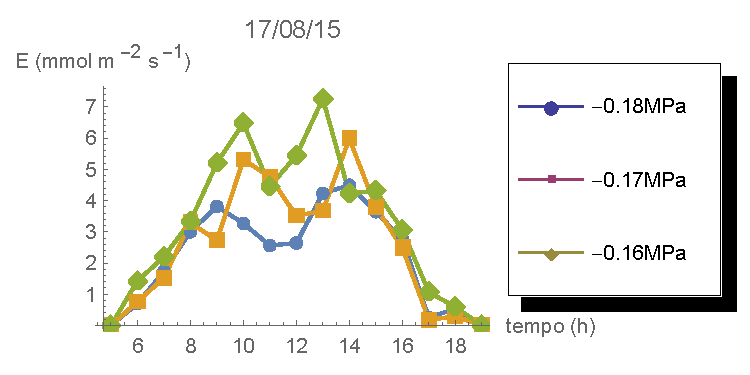
\includegraphics[width=.49\linewidth]{assets/cana/g1_20150817}}
			\subfloat[PAR]{\label{fig:PAR}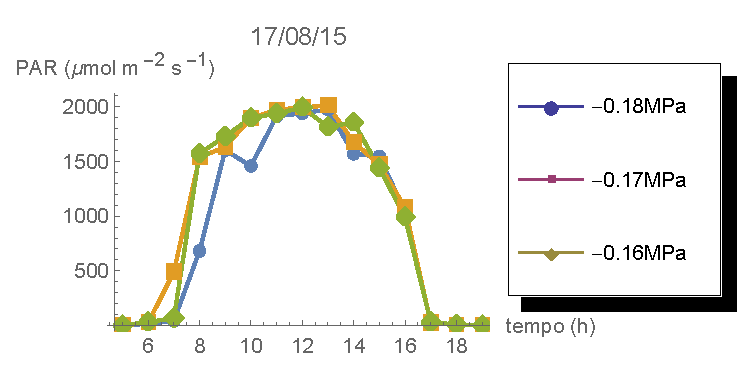
\includegraphics[width=.49\linewidth]{assets/cana/g2_20150817}}\\
			\subfloat[DPV]{\label{fig:DPV}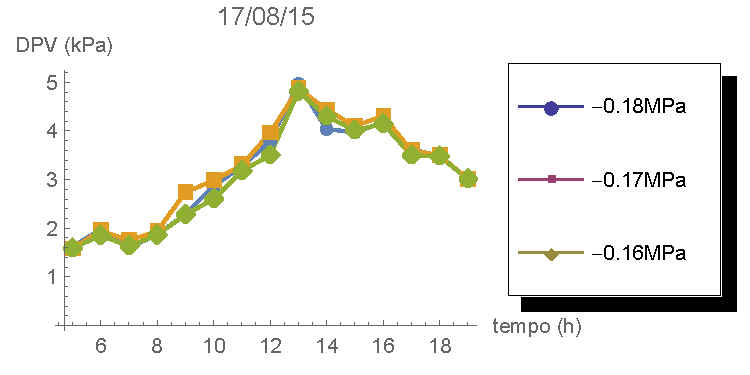
\includegraphics[width=.49\linewidth]{assets/cana/g3_20150817}}
			\subfloat[Transpiração/PAR]{\label{fig:Transpiração/PAR}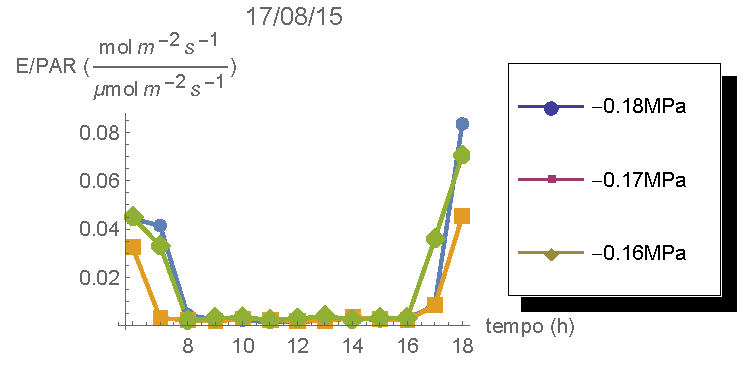
\includegraphics[width=.49\linewidth]{assets/cana/g4_20150817}}\\
			\subfloat[Transpiração/DPV]{\label{fig:Transpiração/DPV}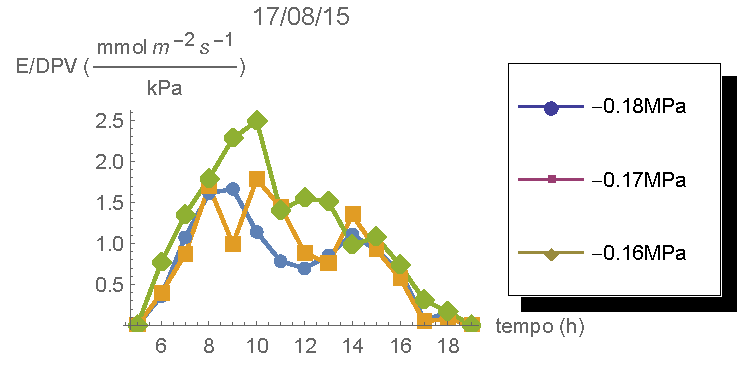
\includegraphics[width=.49\linewidth]{assets/cana/g5_20150817}}
			\caption{Cana de açúcar - 17/08/2015}
			\label{fig:g120150817}
		\end{figure}
		\begin{figure}[H]
			\centering
			\subfloat[Transpiração]{\label{fig:Transpiração}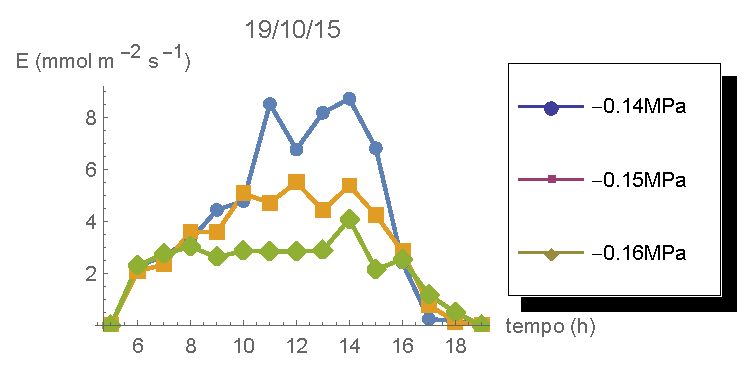
\includegraphics[width=.49\linewidth]{assets/cana/g1_20151019}}
			\subfloat[PAR]{\label{fig:PAR}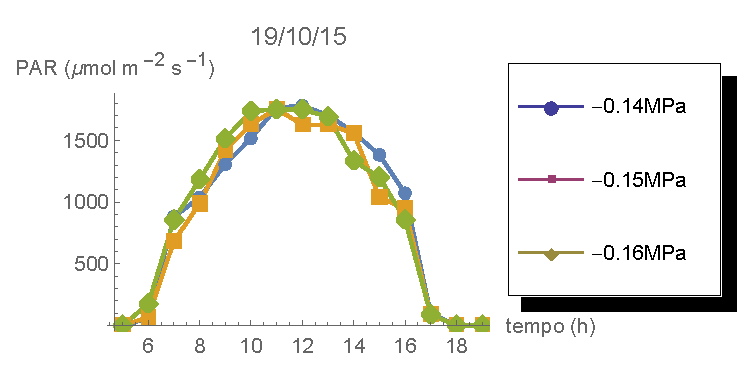
\includegraphics[width=.49\linewidth]{assets/cana/g2_20151019}}\\
			\subfloat[DPV]{\label{fig:DPV}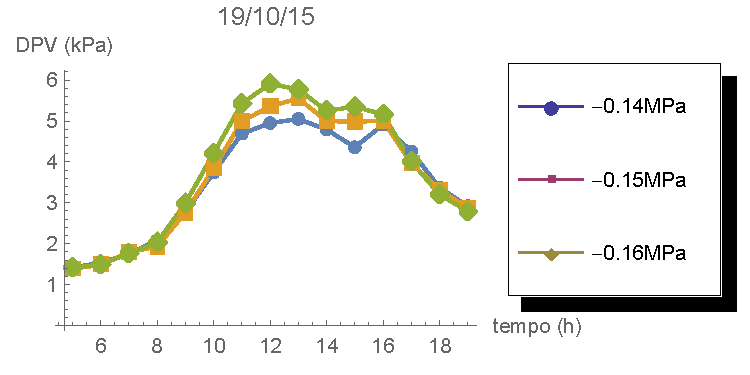
\includegraphics[width=.49\linewidth]{assets/cana/g3_20151019}}
			\subfloat[Transpiração/PAR]{\label{fig:Transpiração/PAR}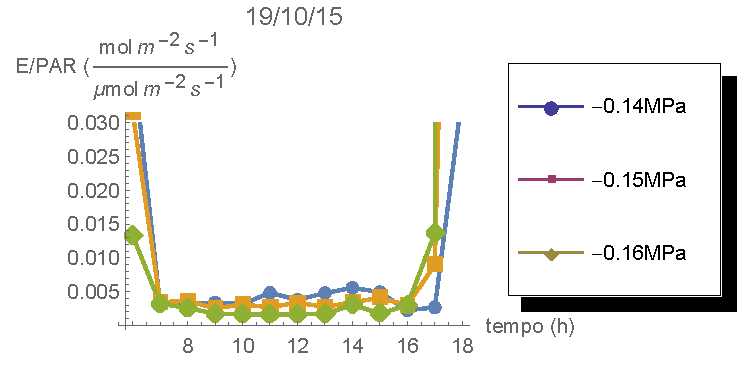
\includegraphics[width=.49\linewidth]{assets/cana/g4_20151019}}\\
			\subfloat[Transpiração/DPV]{\label{fig:Transpiração/DPV}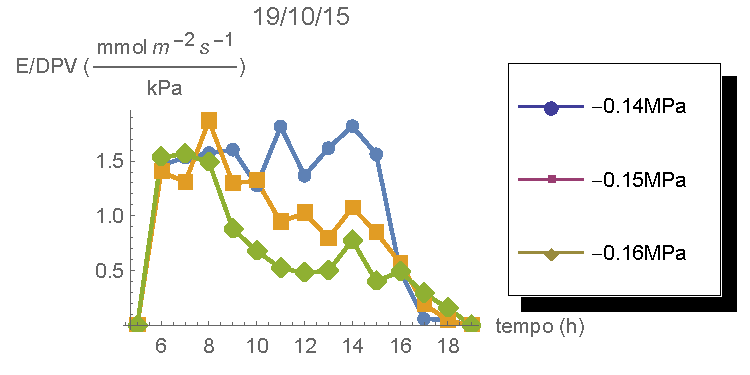
\includegraphics[width=.49\linewidth]{assets/cana/g5_20151019}}
			\caption{Cana de açúcar - 19/10/2015}
			\label{fig:g120151019}
		\end{figure}
	\section{Pata de vaca}
		\begin{figure}[H]
			\centering
			\subfloat[Transpiração]{\label{fig:Transpiração}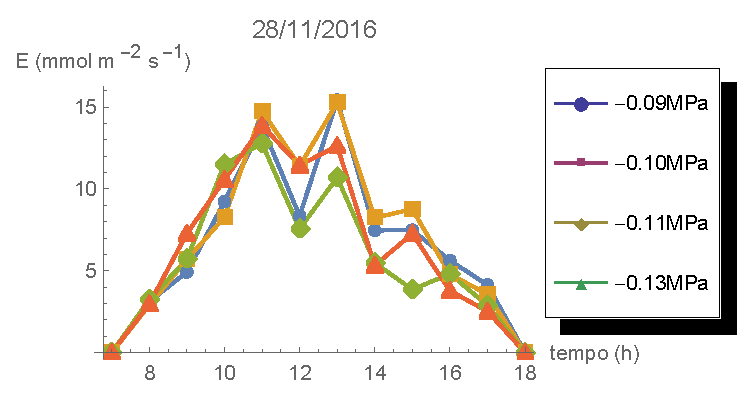
\includegraphics[width=.49\linewidth]{assets/pata/g1_20161128}}
			\subfloat[PAR]{\label{fig:PAR}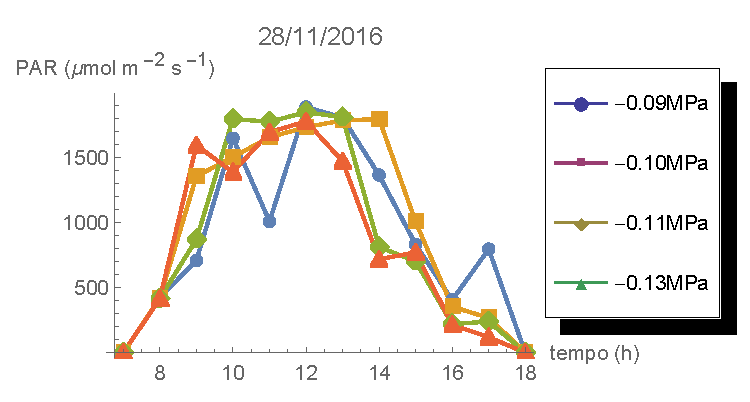
\includegraphics[width=.49\linewidth]{assets/pata/g2_20161128}}\\
			\subfloat[DPV]{\label{fig:DPV}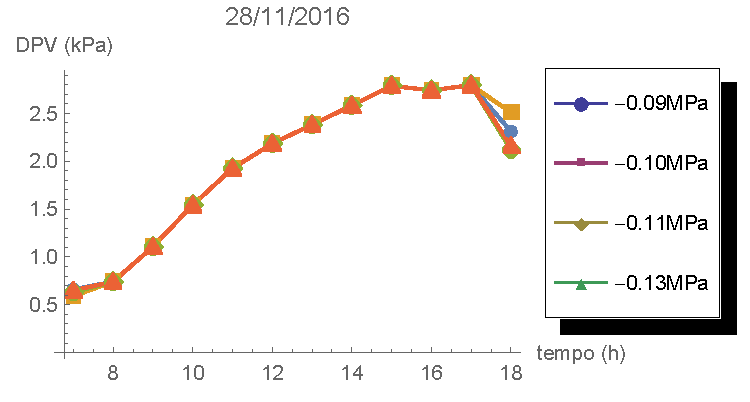
\includegraphics[width=.49\linewidth]{assets/pata/g3_20161128}}
			\subfloat[Transpiração/PAR]{\label{fig:Transpiração/PAR}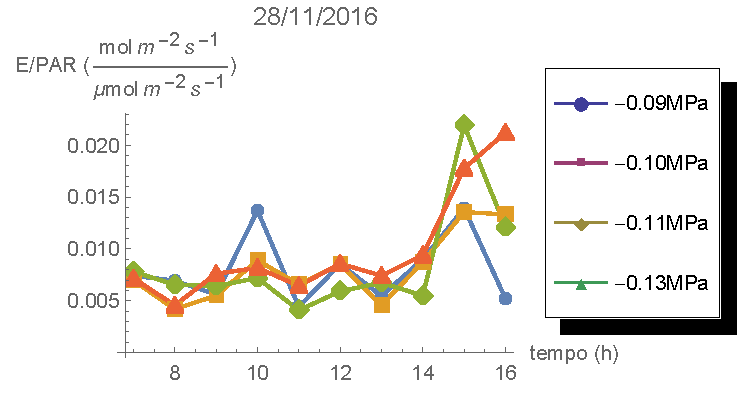
\includegraphics[width=.49\linewidth]{assets/pata/g4_20161128}}\\
			\subfloat[Transpiração/DPV]{\label{fig:Transpiração/DPV}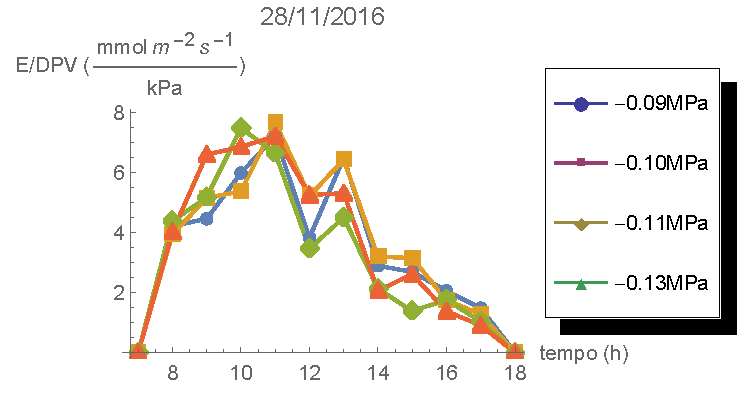
\includegraphics[width=.49\linewidth]{assets/pata/g5_20161128}}
			\caption{Pata de Vaca - 28/11/2016}
			\label{fig:g120161128}
		\end{figure}
	\section{Myrtaceae}
		\begin{figure}[H]
			\centering
			\subfloat[Transpiração]{\label{fig:Transpiração}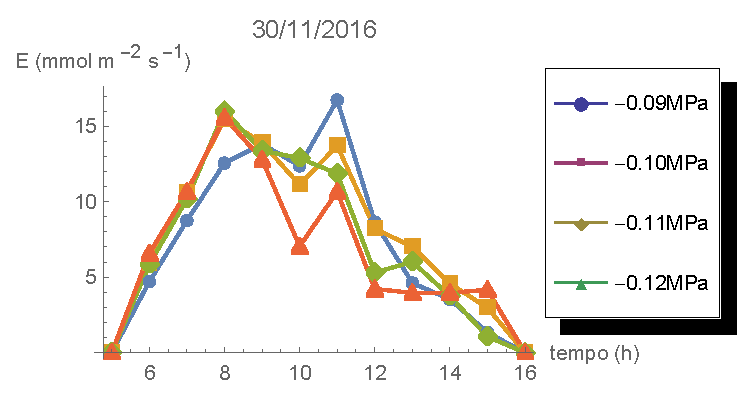
\includegraphics[width=.49\linewidth]{assets/myrtaceae/g1_20161130}}
			\subfloat[PAR]{\label{fig:PAR}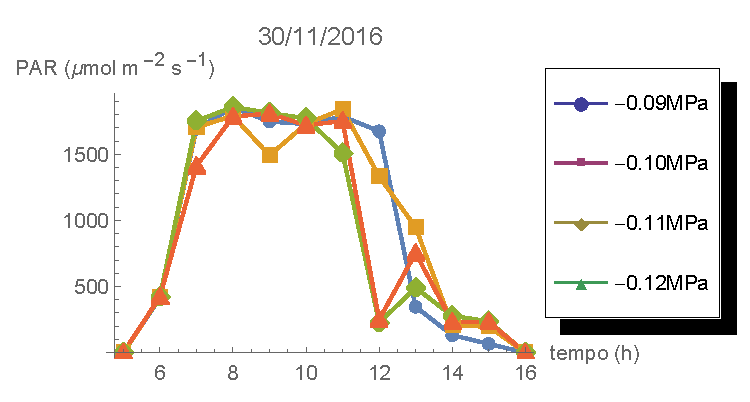
\includegraphics[width=.49\linewidth]{assets/myrtaceae/g2_20161130}}\\
			\subfloat[DPV]{\label{fig:DPV}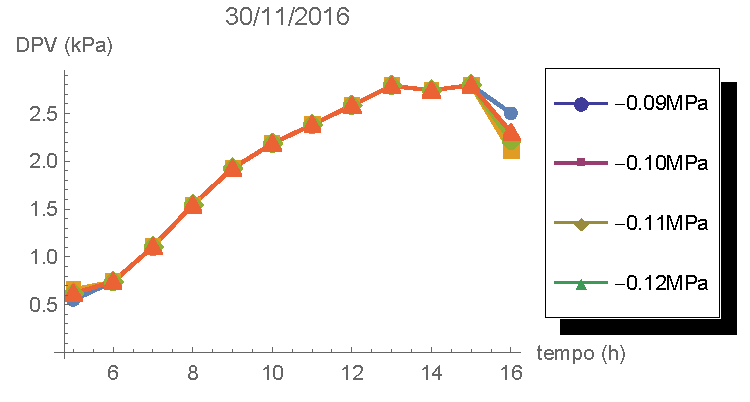
\includegraphics[width=.49\linewidth]{assets/myrtaceae/g3_20161130}}
			\subfloat[Transpiração/PAR]{\label{fig:Transpiração/PAR}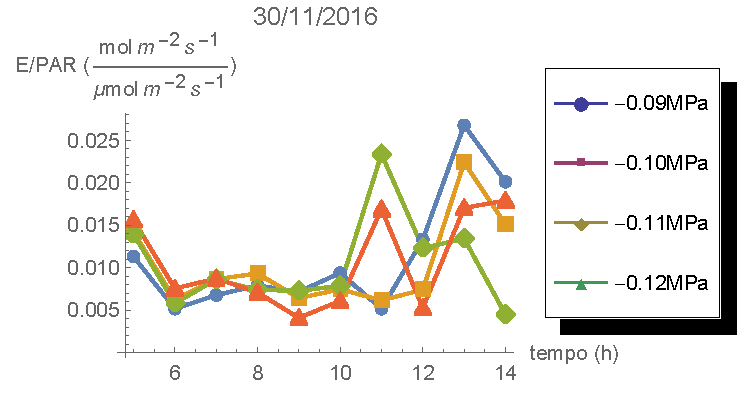
\includegraphics[width=.49\linewidth]{assets/myrtaceae/g4_20161130}}\\
			\subfloat[Transpiração/DPV]{\label{fig:Transpiração/DPV}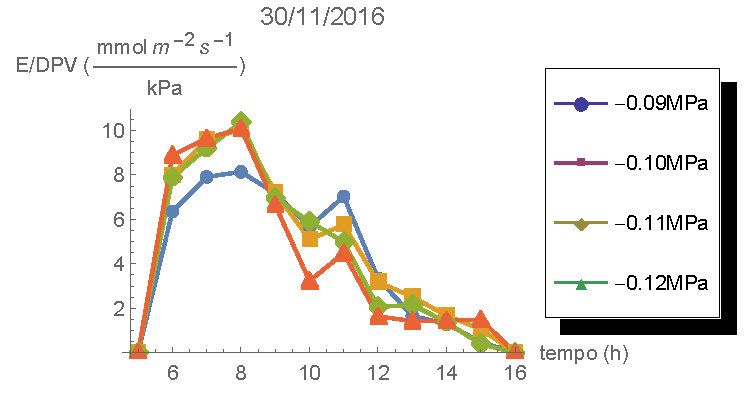
\includegraphics[width=.49\linewidth]{assets/myrtaceae/g5_20161130}}
			\caption{Myrtaceae - 30/11/2016}
			\label{fig:g120161130}
		\end{figure}
	\section{Grumixama}
		\begin{figure}[H]
			\centering
			\subfloat[Transpiração]{\label{fig:Transpiração}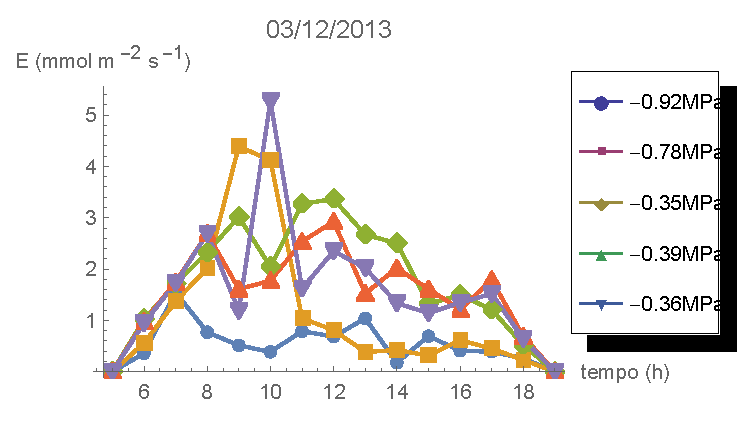
\includegraphics[width=.49\linewidth]{assets/grumixama/g1_20131203}}
			\subfloat[PAR]{\label{fig:PAR}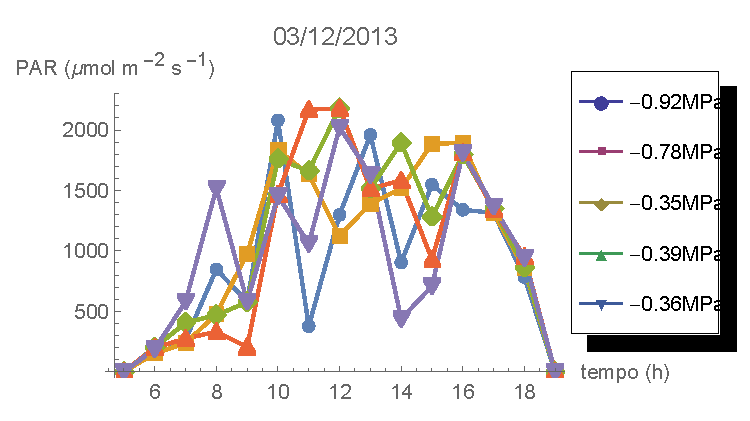
\includegraphics[width=.49\linewidth]{assets/grumixama/g2_20131203}}\\
			\subfloat[DPV]{\label{fig:DPV}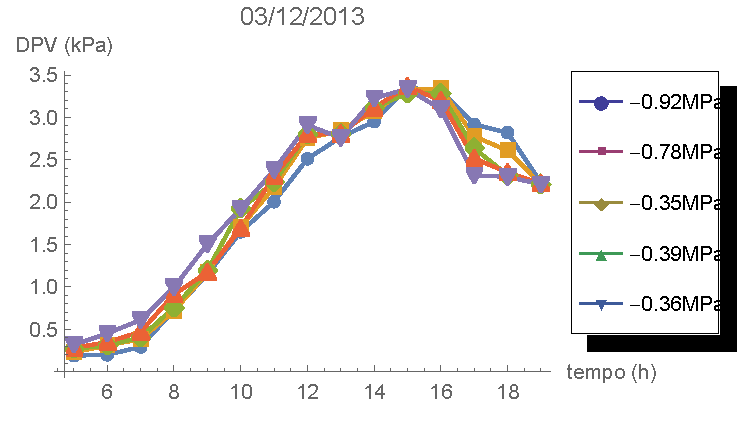
\includegraphics[width=.49\linewidth]{assets/grumixama/g3_20131203}}
			\subfloat[Transpiração/PAR]{\label{fig:Transpiração/PAR}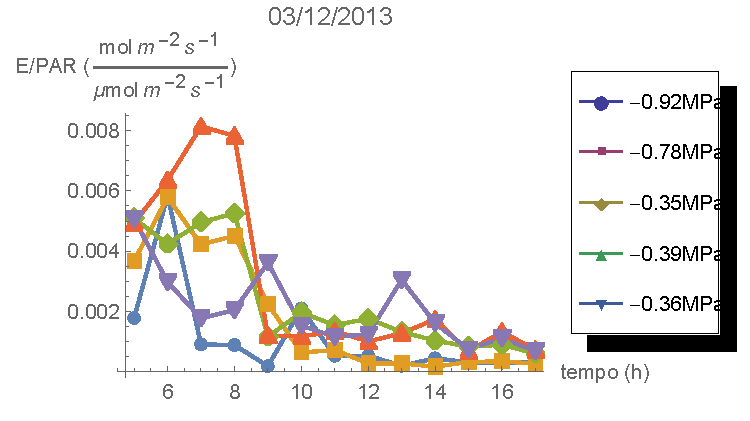
\includegraphics[width=.49\linewidth]{assets/grumixama/g4_20131203}}\\
			\subfloat[Transpiração/DPV]{\label{fig:Transpiração/DPV}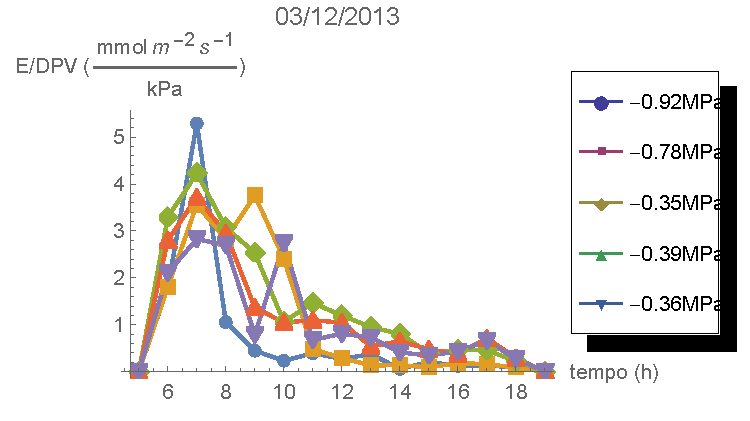
\includegraphics[width=.49\linewidth]{assets/grumixama/g5_20131203}}
			\caption{Grumixama - 03/12/2013}
			\label{fig:g120131203}
		\end{figure}
	\section{Eucalipto}
		\begin{figure}[H]
			\centering
			\subfloat[Transpiração]{\label{fig:Transpiração}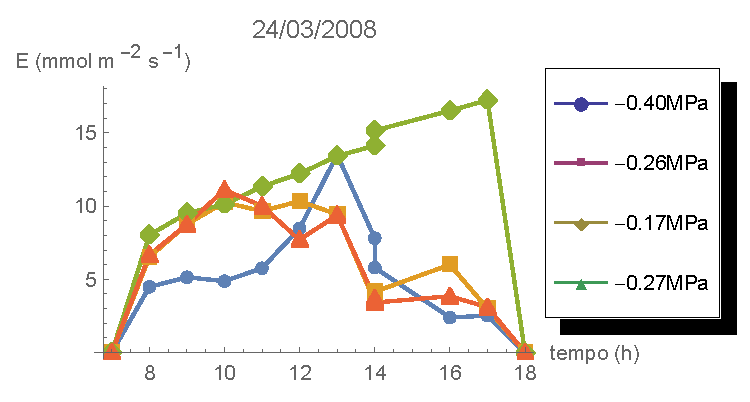
\includegraphics[width=.49\linewidth]{assets/eucalipto/g1_20080324}}
			\subfloat[PAR]{\label{fig:PAR}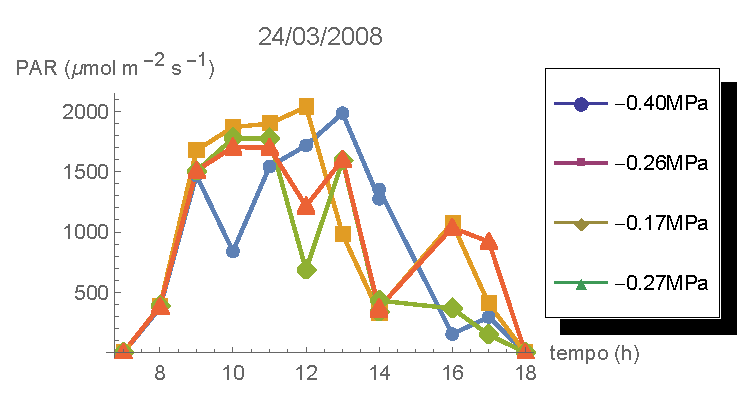
\includegraphics[width=.49\linewidth]{assets/eucalipto/g2_20080324}}\\
			\subfloat[DPV]{\label{fig:DPV}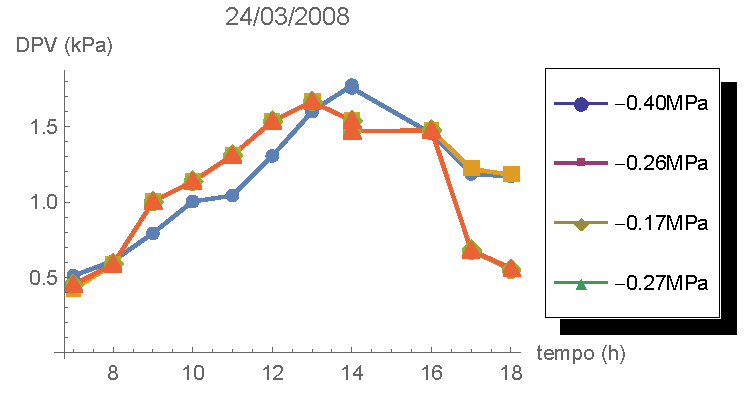
\includegraphics[width=.49\linewidth]{assets/eucalipto/g3_20080324}}
			\subfloat[Transpiração/PAR]{\label{fig:Transpiração/PAR}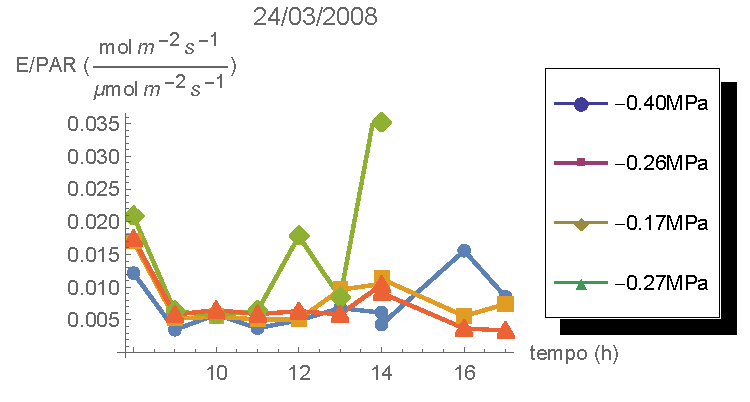
\includegraphics[width=.49\linewidth]{assets/eucalipto/g4_20080324}}\\
			\subfloat[Transpiração/DPV]{\label{fig:Transpiração/DPV}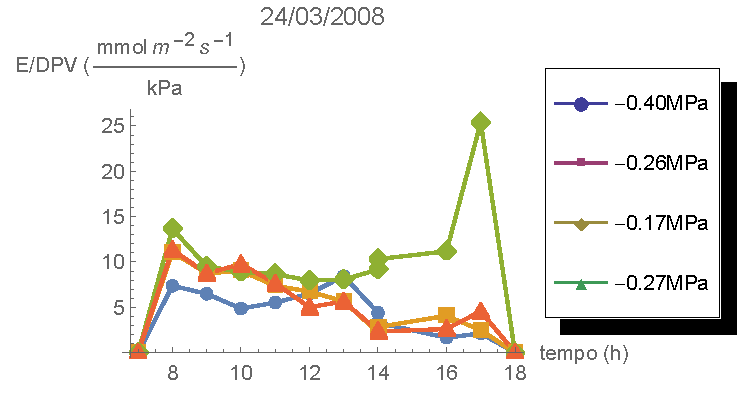
\includegraphics[width=.49\linewidth]{assets/eucalipto/g5_20080324}}
			\caption{Eucalipto - 24/03/2008}
			\label{fig:g120080324}
		\end{figure}
		\begin{figure}[H]
			\centering
			\subfloat[Transpiração]{\label{fig:Transpiração}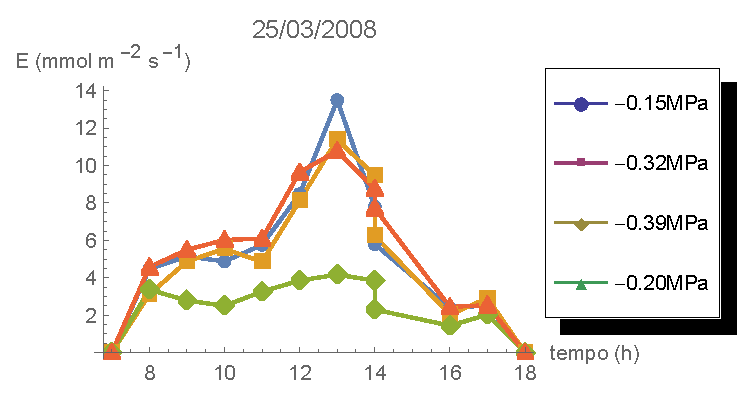
\includegraphics[width=.49\linewidth]{assets/eucalipto/g1_20080325}}
			\subfloat[PAR]{\label{fig:PAR}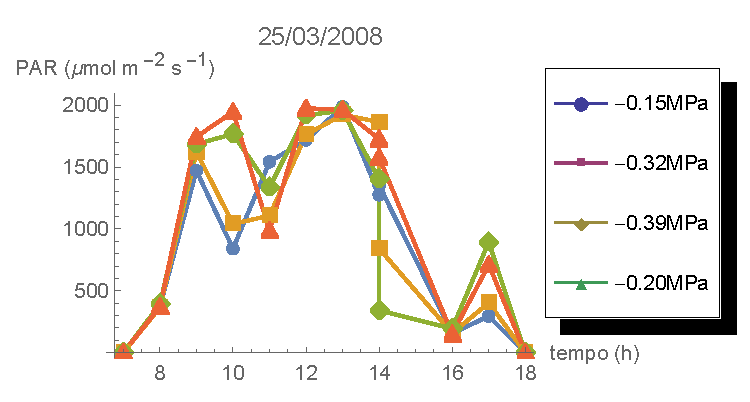
\includegraphics[width=.49\linewidth]{assets/eucalipto/g2_20080325}}\\
			\subfloat[DPV]{\label{fig:DPV}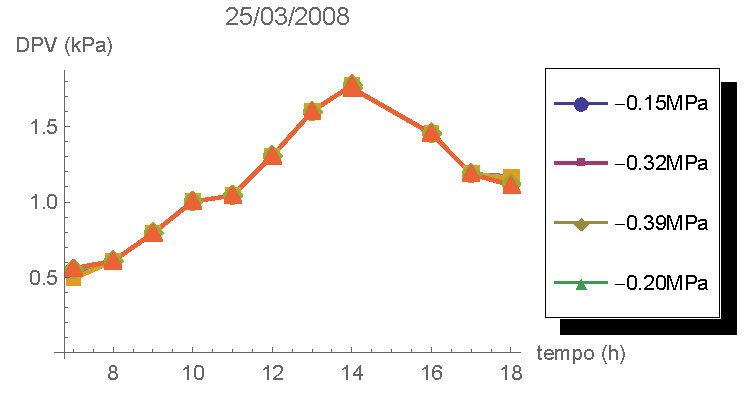
\includegraphics[width=.49\linewidth]{assets/eucalipto/g3_20080325}}
			\subfloat[Transpiração/PAR]{\label{fig:Transpiração/PAR}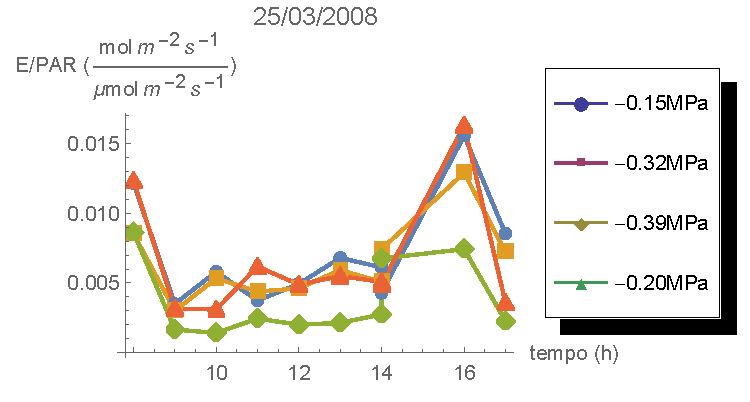
\includegraphics[width=.49\linewidth]{assets/eucalipto/g4_20080325}}\\
			\subfloat[Transpiração/DPV]{\label{fig:Transpiração/DPV}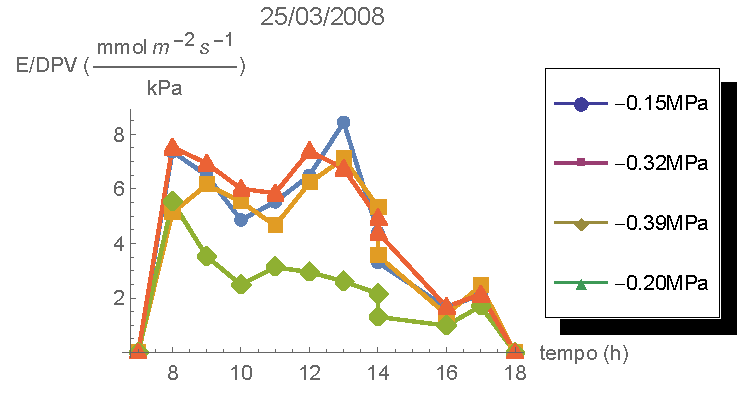
\includegraphics[width=.49\linewidth]{assets/eucalipto/g5_20080325}}
			\caption{Eucalipto - 25/03/2008}
			\label{fig:g120080325}
		\end{figure}
		\begin{figure}[H]
			\centering
			\subfloat[Transpiração]{\label{fig:Transpiração}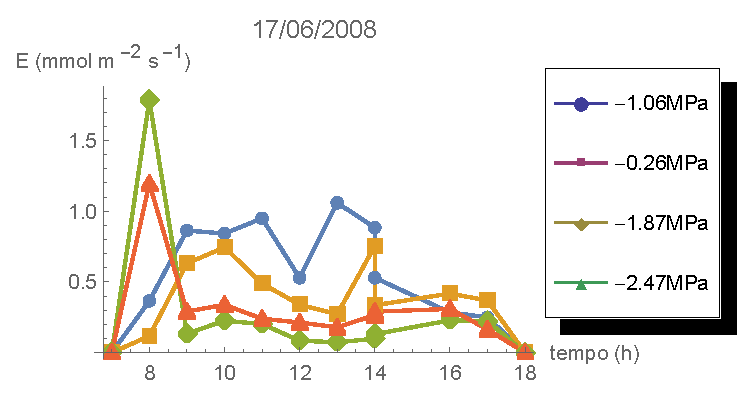
\includegraphics[width=.49\linewidth]{assets/eucalipto/g1_20080617}}
			\subfloat[PAR]{\label{fig:PAR}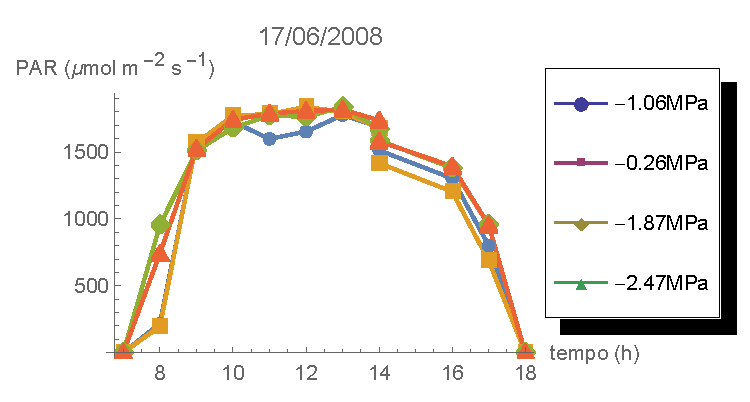
\includegraphics[width=.49\linewidth]{assets/eucalipto/g2_20080617}}\\
			\subfloat[DPV]{\label{fig:DPV}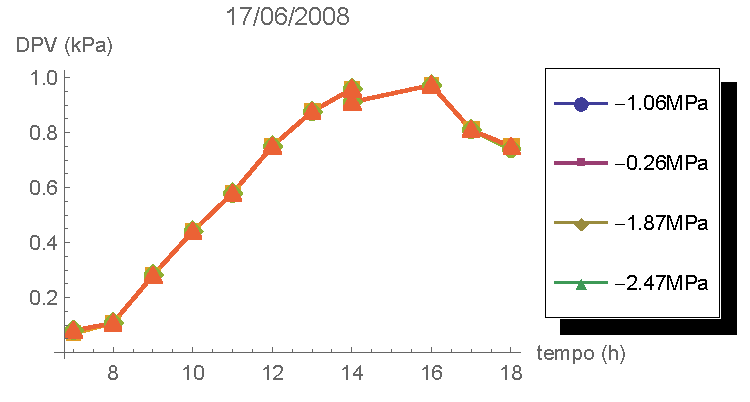
\includegraphics[width=.49\linewidth]{assets/eucalipto/g3_20080617}}
			\subfloat[Transpiração/PAR]{\label{fig:Transpiração/PAR}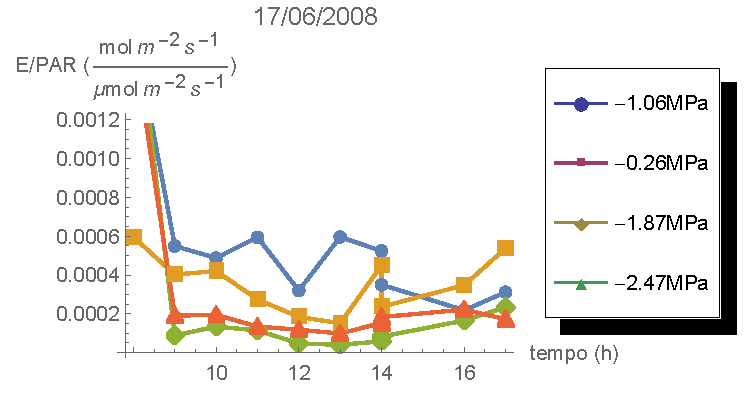
\includegraphics[width=.49\linewidth]{assets/eucalipto/g4_20080617}}\\
			\subfloat[Transpiração/DPV]{\label{fig:Transpiração/DPV}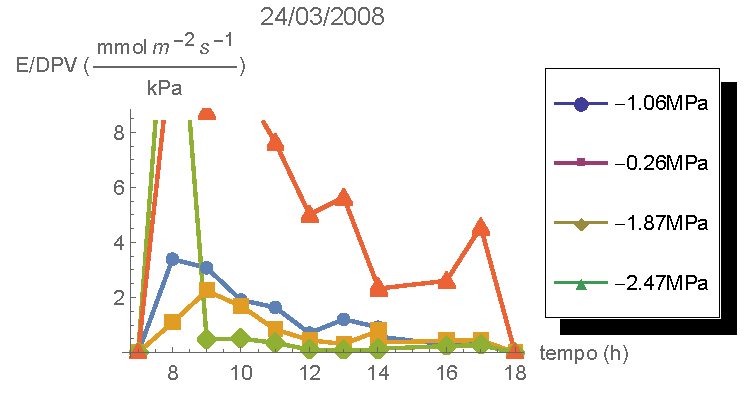
\includegraphics[width=.49\linewidth]{assets/eucalipto/g5_20080617}}
			\caption{Eucalipto - 17/06/2008}
			\label{fig:g120080617}
		\end{figure}
		\begin{figure}[H]
			\centering
			\subfloat[Transpiração]{\label{fig:Transpiração}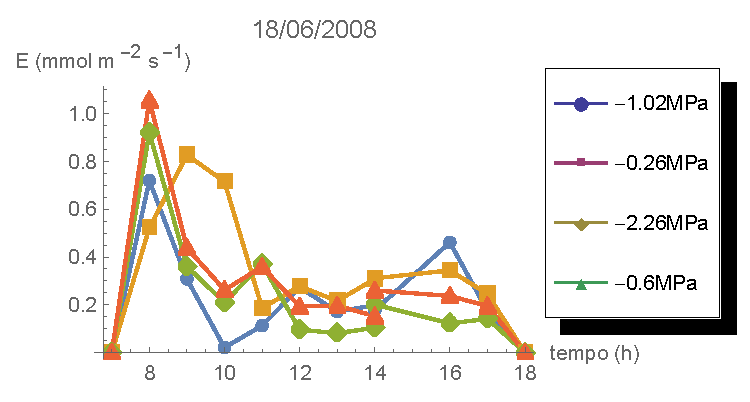
\includegraphics[width=.49\linewidth]{assets/eucalipto/g1_20080618}}
			\subfloat[PAR]{\label{fig:PAR}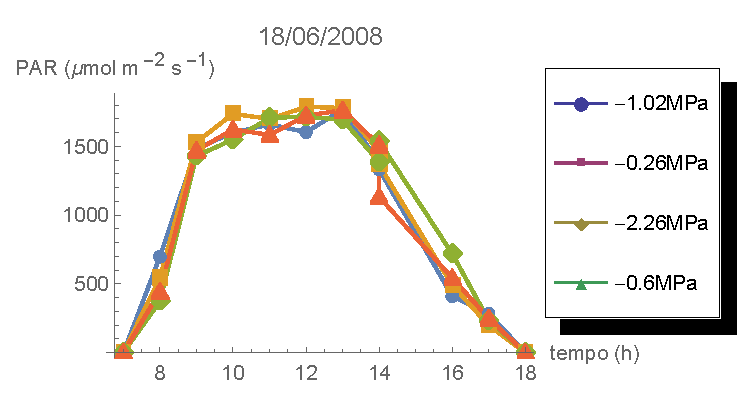
\includegraphics[width=.49\linewidth]{assets/eucalipto/g2_20080618}}\\
			\subfloat[DPV]{\label{fig:DPV}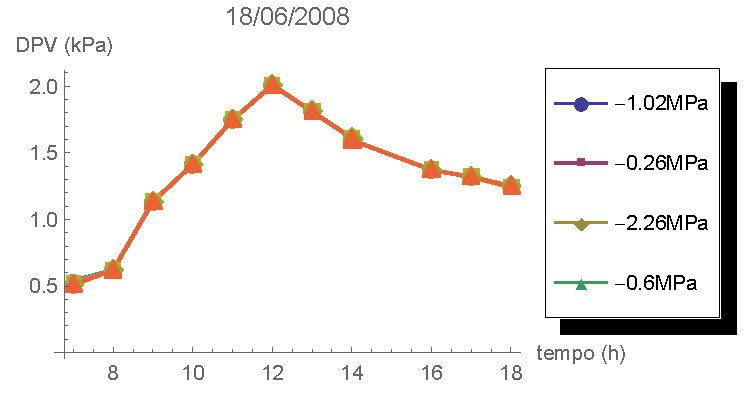
\includegraphics[width=.49\linewidth]{assets/eucalipto/g3_20080618}}
			\subfloat[Transpiração/PAR]{\label{fig:Transpiração/PAR}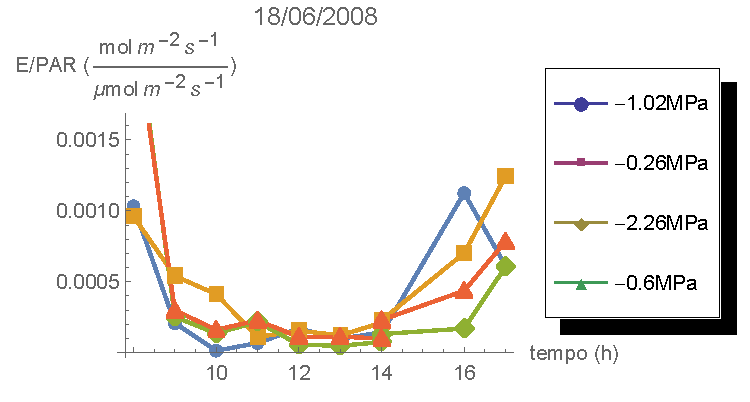
\includegraphics[width=.49\linewidth]{assets/eucalipto/g4_20080618}}\\
			\subfloat[Transpiração/DPV]{\label{fig:Transpiração/DPV}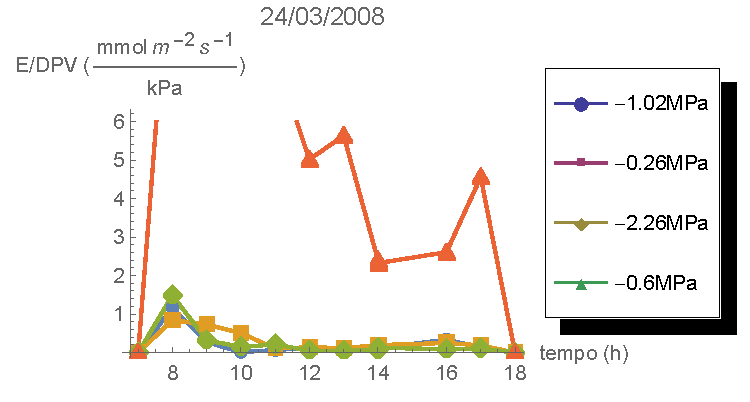
\includegraphics[width=.49\linewidth]{assets/eucalipto/g5_20080618}}
			\caption{Eucalipto - 18/06/2008}
			\label{fig:g120080618}
		\end{figure}
\end{document}